\subsection*{Log ind}
I systemet benyttes en log ind funktion til at beskytte og identificere den enkelte bruger. Brugeren vil her angive log ind information, der vil tillade adgang til information i form af private oplysninger og tidligere resultater, tilknyttet den givne bruger. Aktiviteterne for log ind funktion fremgår af \autoref{fig:logind}.    


\begin{figure} [H]
\centering
\textbf{Aktivitetsdiagram: Log ind}\par\medskip
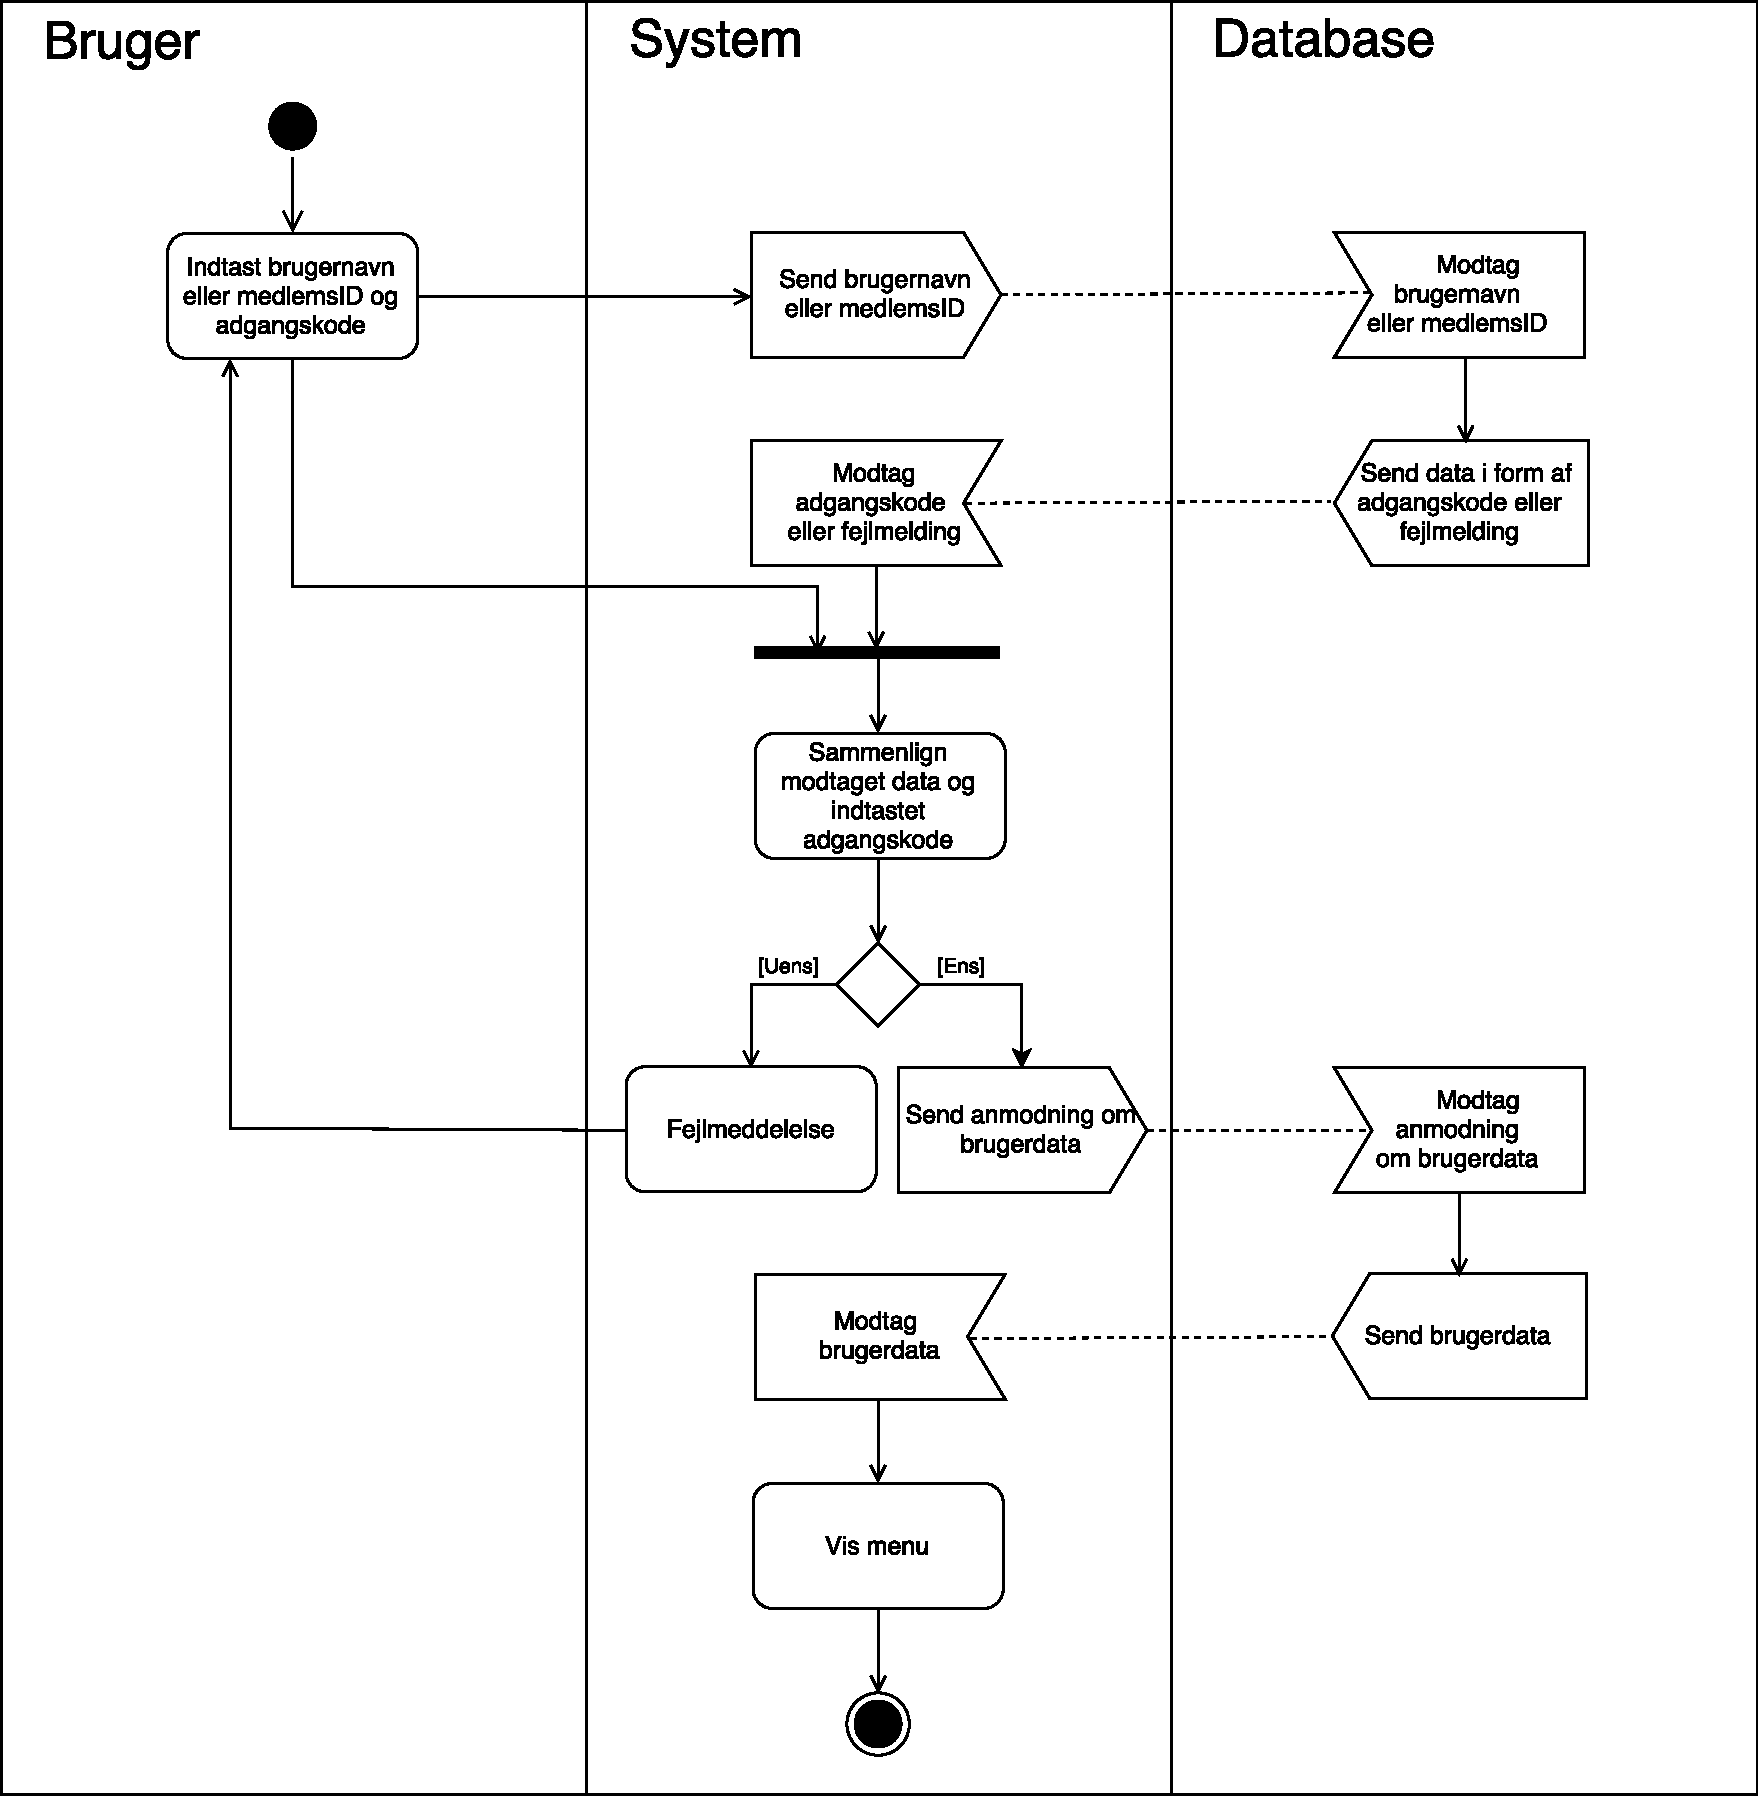
\includegraphics[width=0.9\textwidth]{figures/aktivitetsdiagram/Logind}
\caption{Aktivitetsdiagram over log ind, hvor aktiviteter forekommer hos brugeren, systemet eller databasen.}
\label{fig:logind}
\end{figure}


\noindent
Idet brugeren åbner app'en, vil en grænseflade for log ind vises. Hertil er det ikke muligt at gå videre gennem aktiviteterne, før brugeren har angivet log ind information, i form af medlemsID og en adgangskode. 
Såfremt at medlemsID'et findes, benyttes det efterfølgende i databasen til at identificere den korrekte adgangskode og returnere denne til systemet. Findes medlemsID'et ikke vil dette resultere i at systemet vil vise en fejlmeddelelse, og returnere til grænsefladen for log ind. 
Idet den korrekte adgangskode modtages af systemet, sammenlignes denne med angivet adgangskode. I tilfælde af at adgangskoderne ikke er identiske, vises en fejlmeddelelse og systemet returnere til grænsefladen for log ind. Er adgangskoderne identiske vil systemet hente alt brugerrelateret information fra databasen. I tilfælde af at data'en ikke modtages vises en fejlmeddelelse, ellers tjekkes om det er første gang brugeren logger ind på appen. 
Ved førstegangs log ind vil systemet udføre en aktivitet, hvorigennem systemet får angivet brugerens kategorisering af KOL. Efter angivelsen af kategoriseringen, eller ved efterfølgende log ind vil systemet gå direkte til at vise hovedmenuen.  
    

%Når KOL-patienten vil anvende app'en skal medlemsID eller brugernavn samt kodeord indtastes. Systemet sender det indtastede medlemsID eller brugernavn til databasen, som tilbagesender det tilhørende kodeord, hvis det findes i databasen. Findes de indtastede informationer ikke, sendes en fejlmeddelelse i form af 0. Systemet sammenligner herefter brugerens indtastede adgangskode med adgangskoden fra databasen. Er de to værdier ens, har brugeren indtastet de korrekte informationer, hvortil brugerdata hentes fra databasen og hovedmenuen vises. Brugerdata omfatter brugerens informationer og tidligere resultater. Er de to værdier ikke ens, tilbagesender systemet en fejlmeddelelse, og brugeren får derefter mulighed for at indtaste log ind informationen igen. 